\documentclass[12pt]{article}
\usepackage[letterpaper, total={6in, 8in}]{geometry}
\setlength{\oddsidemargin}{0in}
\setlength{\evensidemargin}{0in}
\setlength{\textwidth}{6.5in}
\setlength{\parindent}{0in}
\setlength{\parskip}{\baselineskip}

\usepackage{amsmath,amsfonts,amssymb}
%\usepackage{subfigure}
\usepackage{sectsty}
\usepackage{multirow}
\usepackage{makecell}
\usepackage{float}
\usepackage[utf8x]{inputenc}
\usepackage[pdftex]{graphicx}
\usepackage[toc,page]{appendix}
\usepackage{enumitem}
\usepackage{indentfirst}
\usepackage{scrextend}
\usepackage{caption}
\usepackage{hyperref}
\usepackage{adjustbox}
\usepackage{subcaption}

%\usepackage{xurl}

\usepackage{listings}
\usepackage{color} %red, green, blue, yellow, cyan, magenta, black, white
\definecolor{mygreen}{RGB}{28,172,0} % color values Red, Green, Blue
\definecolor{mylilas}{RGB}{170,55,241}

\DeclareFixedFont{\ttb}{T1}{txtt}{bx}{n}{10} % for bold
\DeclareFixedFont{\ttm}{T1}{txtt}{m}{n}{10}  % for normal

\usepackage{color}
\definecolor{deepblue}{rgb}{0,0,0.5}
\definecolor{deepred}{rgb}{0.6,0,0}
\definecolor{deepgreen}{rgb}{0,0.5,0}

\usepackage{sectsty}

\sectionfont{\fontsize{14}{15}\selectfont}
\subsectionfont{\fontsize{12}{15}\selectfont}

\usepackage{listings}
\lstset{language=Matlab,%
	%basicstyle=\color{red},
	breaklines=true,%
	morekeywords={matlab2tikz},
	keywordstyle=\color{blue},%
	morekeywords=[2]{1}, keywordstyle=[2]{\color{black}},
	identifierstyle=\color{black},%
	stringstyle=\color{mylilas},
	commentstyle=\color{mygreen},%
	showstringspaces=false,%without this there will be a symbol in the places where there is a space
	numbers=left,%
	numberstyle={\tiny \color{black}},% size of the numbers
	numbersep=9pt, % this defines how far the numbers are from the text
	emph=[1]{for,end,break},emphstyle=[1]\color{red}, %some words to emphasise
	%emph=[2]{word1,word2}, emphstyle=[2]{style},    
}


% Python style for highlighting
\newcommand\pythonstyle{\lstset{
		language=Python,
		basicstyle=\ttm,
		otherkeywords={self},             % Add keywords here
		keywordstyle=\ttb\color{deepblue},
		emph={MyClass,__init__},          % Custom highlighting
		emphstyle=\ttb\color{deepred},    % Custom highlighting style
		stringstyle=\color{deepgreen},
		frame=tb,                         % Any extra options here
		showstringspaces=false            % 
}}


% Python environment
\lstnewenvironment{python}[1][]
{
	\pythonstyle
	\lstset{#1}
}
{}

% Python for external files
\newcommand\pythonexternal[2][]{{
		\pythonstyle
		\lstinputlisting[#1]{#2}}}

% Python for inline
\newcommand\pythoninline[1]{{\pythonstyle\lstinline!#1!}}


\begin{document}
\hfill Sam Feig $|$ Vladimir Zhdanov \\
\textbf{Photo Sorter Final Project Report}\hfill CSCI 4831/5722 \\
\rule{\textwidth}{.75pt}

\section{Introduction}
	With the unprecedented increase of digital media in the past few decades, the number of photographs in existence has grown exponentially as time has passed. With film photography, each image was precious, taking up valuable space on a roll. But with digital photographs, this limitation is essentially gone, and people can now take a nearly unlimited number of photographs at any moment. Photos come off the camera, and are stored in a hard drive, un-clustered and forgotten. Thus, the goal of this project is to make a photo sorter which will be able to group similar, or near-duplicate, images to find that "perfect shot".

\subsection{Project Goals}
	With this project, we hope to design a photo sorter with a simple user interface. The user will be able to select a group of photos as input. With the input, we hope to use object detection to find images containing only specific things (such as people, cars, etc.), and to filter our input based on these. Finally, the program will be able to simply sort the selected images by similarity, organizing the cluttered input into a nice clustered output.

\subsection{Approach}
	In order to build a near-duplicate photo sorter, we decided to use feature detection to match similar images together. We believe that near-duplicate images will have a high number of matching features, and we will be able to have the user decide a threshold on how many matching features will be considered a near-duplicate image. 
	
	To detect objects in the images, we plan to use a pre-trained neural network, trained to detect common objects in context. We plan to use a fast model which can be used in real-time image detection, since we want to be able to quickly detect objects for a large number of input images in a short amount of time. We plan find a model which is fairly resource efficient, despite likely sacrificing some accuracy, to help with the overall performance of our application.
	
	We believe that with this approach we can get decent accuracy without hurting the overall run-time significantly. The feature detection will work well, but will greatly depend upon the threshold that we set for what is a match. When this threshold is set intelligently, it should produce results that are fairly accurate with minimal error.

\section{Computer Vision Methods}
\subsection{Near Duplicate Matching}
	We tried to use two different feature detection algorithms in our project. First was Scale-Invariant Feature Transform (SIFT), and the other was Oriented FAST and Rotated BRIEF (ORB). We tried using ORB as it was branded as an open source alternative to SIFT or SURF by OpenCV. Both are implemented in the code but only SIFT is actively used due to issues encountered with ORB.
	
	In the end, our near duplicate photo sorting algorithm uses Scale-Invariant Feature Transform (SIFT) to do keypoint and description generation for the features in the image. In OpenCV's SIFT implementation, feature descriptors are a matrix of neighbors to the feature pixel. These can then be matched using a nearest neighbors algorithm to determine feature matches. 
	
	OpenCV has a brute force matcher (BFBatcher), and a Fast Library for Approximate Nearest Neighbors matcher (FLANN). Our program's feature matching uses a FLANN based matcher to compute feature descriptor matches due to the increased speed that FLANN provides on large data sets with high dimensional features. We are using FLANN with the FLANN\_INDEX\_KDTREE algorithm and 5 trees. FLANN runs k-nearest neighbors with $k=2$ on the descriptors for the two images it is passed and returns a list (in this case of the best 2) descriptors that matched for each descriptor from a feature in the first image.
	
	From this list of feature matches, they get narrowed down using a ratio test, eliminating all but the best feature matches with a ratio of 0.7 (ie: our best match must be  sufficiently different from the second match to keep it). This helps to prevent ambiguous matching of features, improving accuracy.
	
	This enables us to have a robust near duplicate matcher while gaining some performance benefits over a brute force solution. We were unable to get the ORB descriptors to work effectively with similar levels of accuracy as SIFT. This prevented us from making use of ORB's design for mobile devices and real time feature detection that would have sped up runtime of the program in a similar way that we managed with our object detection neural net.
	
	
\subsection{Object Detection}
	We tried several different methods for object detection before settling on the network used in the final product. Our initial idea was to try to use the convolutional neural network which would produce the highest confidence in our detected objects. We attempted object detection with a pre-trained VGG-16 model, which is a top of the line deep convolutional neural network boasting over 90\% accuracy in object detection tasks. While this model was successfully able to detect objects in our images, we noticed that the operational runtime was extremely slow and even to process a single image would take upwards of 30 seconds. Thus, for the use case of the photo sorter application needing to process many images, we needed to find a faster alternative.
	
	A faster alternative for image detection was the You Only Look Once (YOLO) model. This algorithm is often used in real-time image detection, able to process over 150 frames per second in some instances. While YOLO is one of the fastest object classification models, there is a large trade-off on accuracy due to its processing speed (around 64\% mean accuracy), and it ended up miss-classifying a lot of objects in our images.
	
	For this photo sorter, we found a good balance between accuracy and speed in Single Shot Detectors (SSDs), which are faster than normal CNNs as they only need to take a single shot to classify multiple objects in an image. Specifically, we made use of a MobileNet SSD, which is a model that is traditionally meant for resource constrained devices such as smart-phones. For our use case, we found that using this network allowed our application to be more lightweight and for the object detection to run in a reasonably short amount of time. This specific MobileNet SSD was pre-trained on the Common Objects in Context dataset, and fine-tuned on the PASCAL Visual Object Classes dataset to get a mean average precision of around 72\%. This model allowed us to detect 20 general objects (such as people, cars, boats, etc.) with a good balance of precision and efficiency, while also not being very resource intensive to run in our application.
	

\subsection{Limitations and Future Extensions}
	One major limitation of our implementation of the near duplicate matching is in its run time. Despite using the faster FLANN based matcher for kNN, the algorithm still takes a long time to run for checking each image against another (which has to be done many times). This means that the more images it must check, the longer the program will need to run to do the matching for each image. 
	
	In addition, when attempting to use the apparently more efficient algorithm ORB, we hit issues with it not producing enough feature matches to effectively match images together. It produces feature matches numbering in the 20-150 range, whereas when matching an image using SIFT features, it typically had between 600-50,000 feature matches depending on the image. This meant that accuracy with ORB was a problem and lead to a lot of miss-matching of images when doing the nearest neighbor matching.

	To attempt to fix the issue of slow runtime, we implemented two different versions of the matching algorithm, one that used a dictionary of matched images and the other that used a matrix. The dictionary was fast as it would eliminate checking an image against any others once it had been matched once. Though this had the trade off that if the cutoff threshold for a match was changed, all the data would have to be recomputed as that threshold determined when images were eliminated from the algorithm. The matrix method had a couple qualities that we liked despite it having much worse performance in terms of processing time. In the matrix method, we compute an upper triangular matrix of all the numbers of matches between the different combinations of images. This allows us to re-sort/filter the data when changing the match threshold without needing to recompute any of the values in the matrix. Because our algorithm was designed to save the data to a pickled file once it was computed, this had the advantage of speeding up tuning of that threshold and future sorting at the expense of a drastically increased initial run-time. 
	
	Our biggest improvement we could make in the future would be to multi-thread the matrix method. Since each row of the matrix is independent, they can be run individually then combined afterwards. Adding this multi-threading to the matrix method would drastically increase run-time performance while giving the benefits of not needing to recompute data. As will be seen in the results of the runtime analysis, if we could speed up the initial matrix computation it would make this method far superior as it will have the best features of both versions of the algorithm.

	
	
	A limitation of our object detection method is the number of objects which we are able to detect. The network we are using is trained to detect 20 general classes of objects, but is not able to detect them in detail. For example, the network can detect a car but not its model, or it can detect a cat without the breed. If we want to be able to detect more types of objects in the future, additional training and fine tuning of the model would be necessary to do so.
	
	Another limitation of the object detection model is its ability to detect certain subsets of classes of objects. For example, the model is able to detect lighter-skinned people with much higher confidence than those with darker skin. In the provided image set, a good example of this is between the images \texttt{paris\_general\_000001.jpg} and \texttt{paris\_general\_000008.jpg}. The white man in the first image is detected with over 99\% confidence by the model, while the darker skinned people in the second image are found with at most 49\% confidence by the model. This is likely a result of the data used to train the model with, and could be improved with additional training and adjustments.
	
	\begin{figure}[H]
		\centering
		\begin{subfigure}[b]{.5\textwidth}
			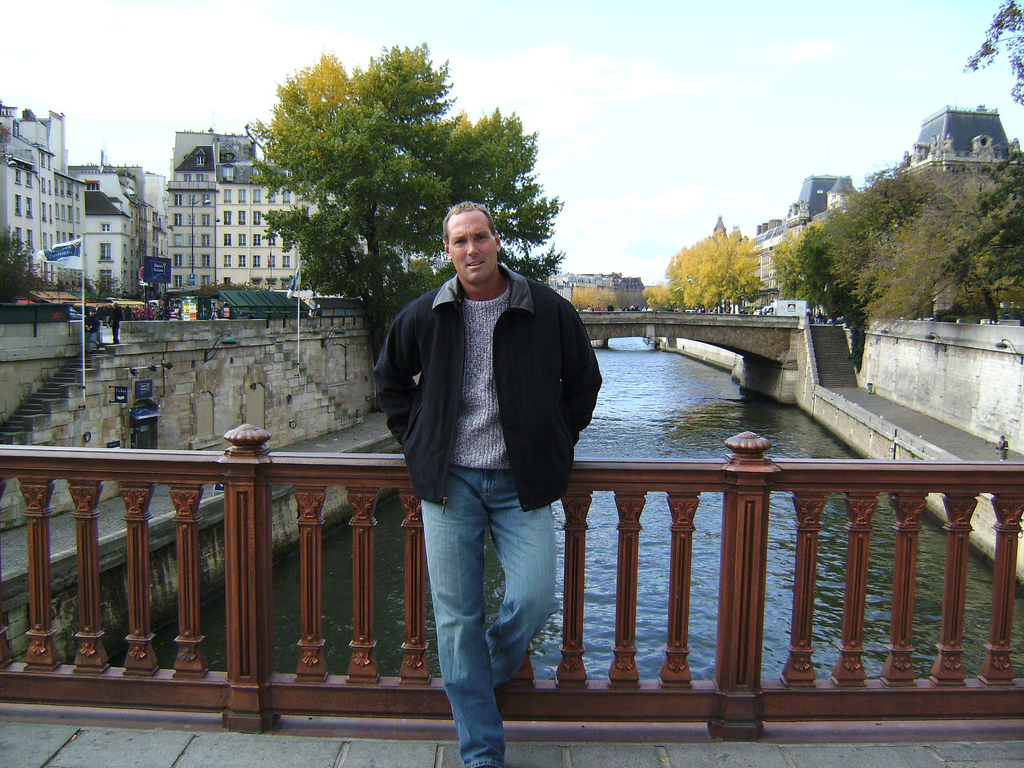
\includegraphics[width=1\textwidth]{images/paris_general_000001.jpg}
		\end{subfigure}%
		~
		\begin{subfigure}[b]{.5\textwidth}
			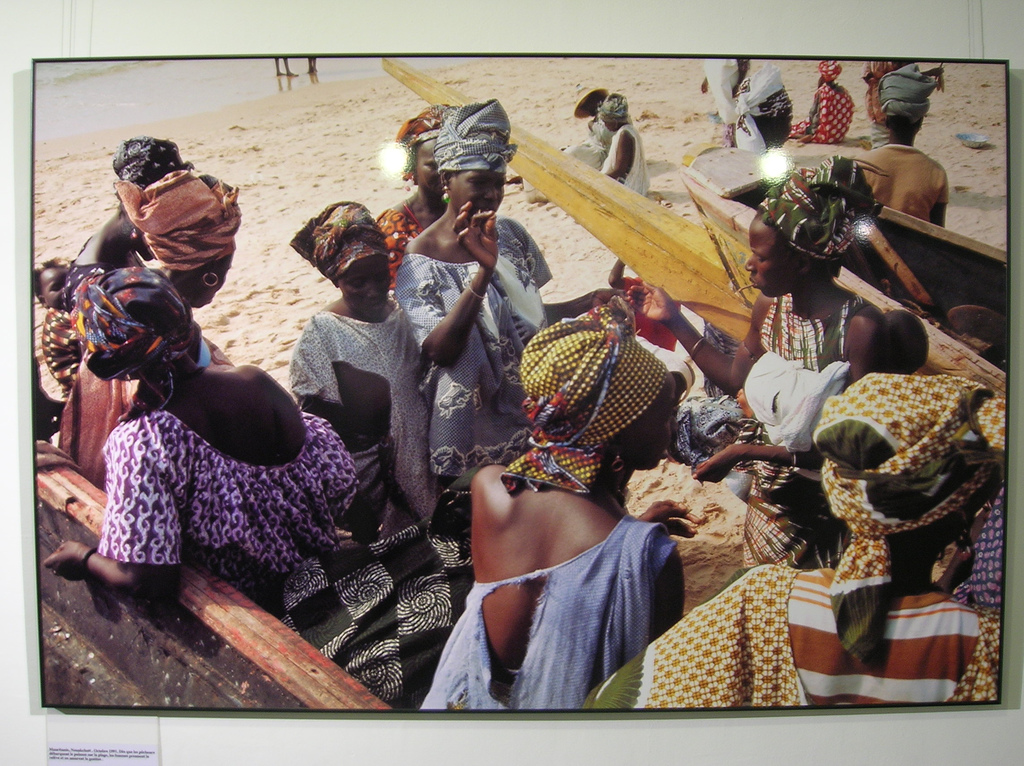
\includegraphics[width=1\textwidth]{images/paris_general_000008.jpg}
		\end{subfigure}
		
		\caption{\texttt{paris\_general\_000001.jpg} (left) and \texttt{paris\_general\_000008.jpg} (right).}
		\label{fig:poor_subset_detection}
	\end{figure}
	
\section{Results}
Our final application is a simple GUI which can be used to load images, detect objects in images, filter images by those objects, and ultimately sort near-duplicate photos into separate directories. This application is made to be very customizable, with many of the detection and sorting parameters being able to be adjusted. The user can choose the object detection confidence, which objects to include or filter out, and the features matched threshold for an image to be considered a near-duplicate. Also, the features and matches can be saved so that these parameters can be adjusted without a long re-computation time. A detailed walk-through of the full functionality of the application can be seen in the \texttt{README} included alongside the code of this project.

\subsection{Object Classification}
The convolutional neural network is able to successfully classify 20 classes of objects including people, cars, and boats. The object detection is quite fast, and can detect all of the specified objects in all of the images provided to the program. Figure \ref{fig:correct_classification} shows an example of a correct classification.
\begin{figure}[H]
	\centering
	\includegraphics[width=.9\textwidth]{images/successful_classification_person.png}
	\caption{An example of a correct classification. The man on the bridge is successfully classified as \texttt{person} with $99.95\%$ confidence.}
	\label{fig:correct_classification}
\end{figure}

Due to the model chosen for this object classification task, along with the data it was trained on, we see that it is not always entirely accurate. Generally, these detections are fairly accurate, and give a good baseline for quickly detecting a certain type of object in a large group of images for image sorting. Figure \ref{fig:incorrect_classification} shows an example of an incorrect classification, where the Eiffel Tower is mistakenly classified as a boat. We believe this is due to the Eiffel Tower looking like the mast of a ship, and it is surrounded by blue sky so it may seem to be like a boat on the ocean. With more fine tuning, it may be possible to reduce these misclassifications.

\begin{figure}[H]
	\centering
	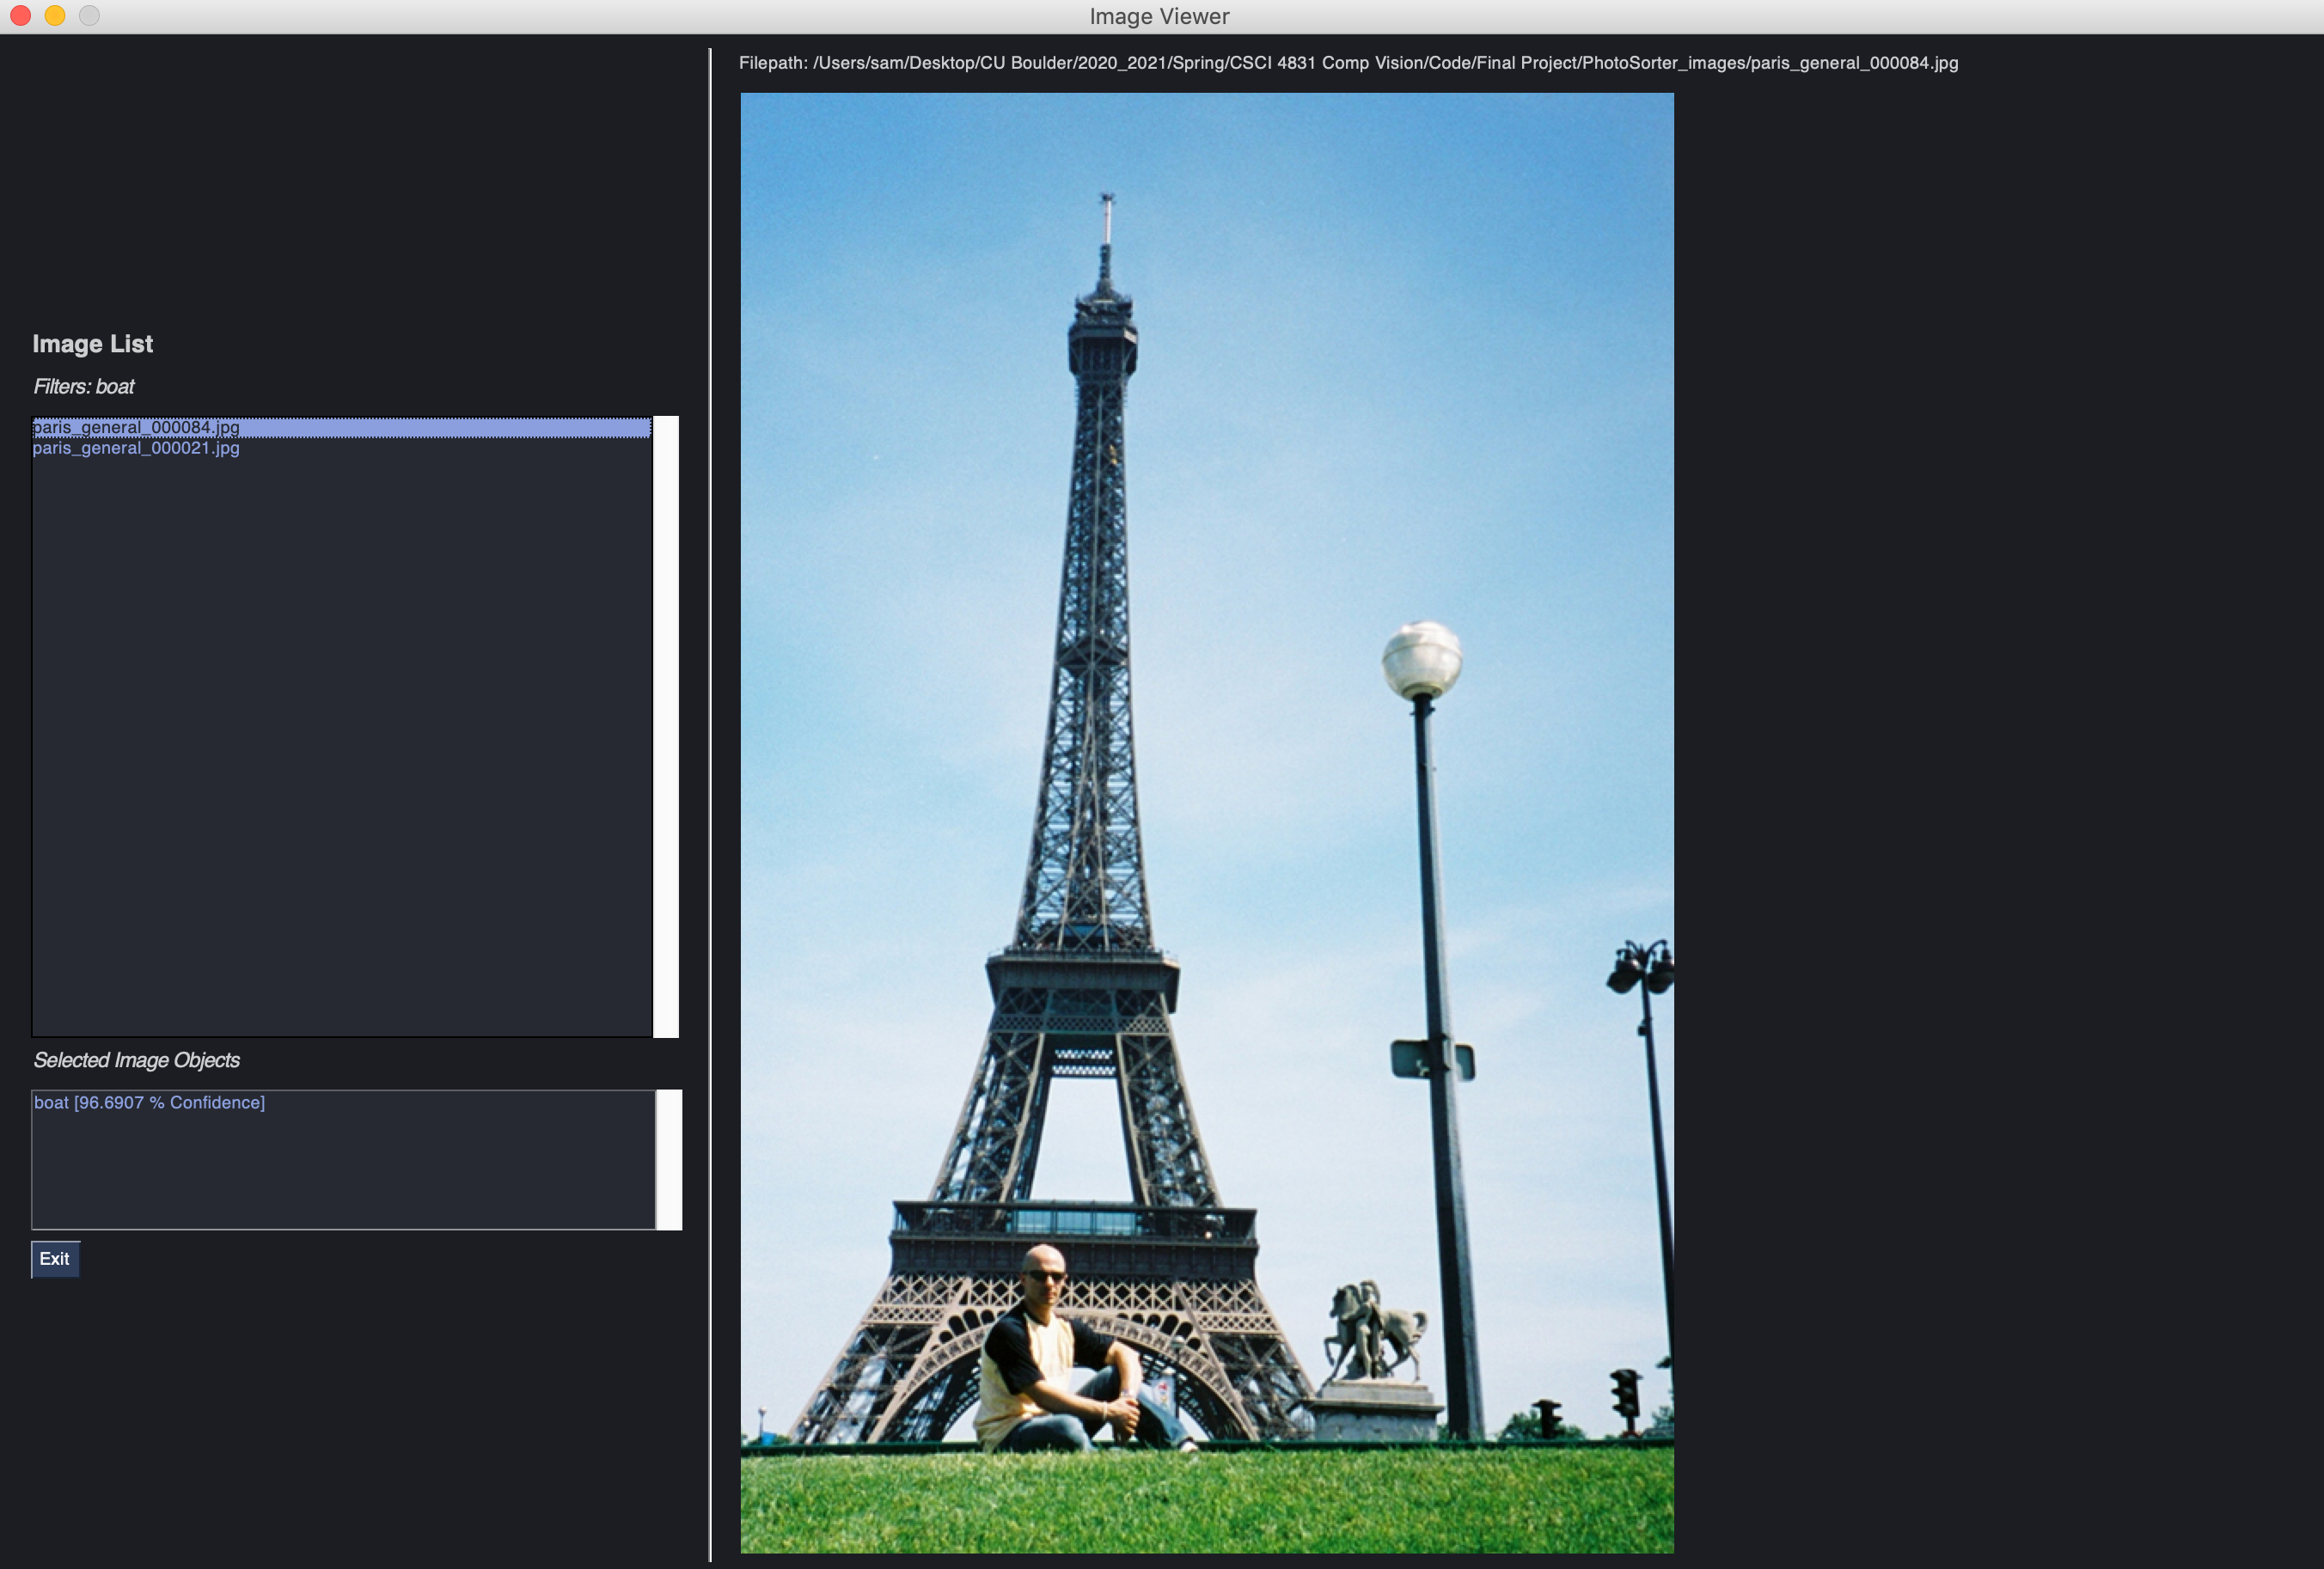
\includegraphics[width=.9\textwidth]{images/incorrect_classification_boat.png}
	\caption{An example of an incorrect classification. The Eiffel Tower is incorrectly classified as a \texttt{boat} with $96\%$ confidence.}
	\label{fig:incorrect_classification}
\end{figure}

\subsection{Image Sorting Results}
To help mitigate long running times, our program includes an output showing the progress of our feature computation and matching. This part of our GUI is shown in Figure \ref{fig:sort_gui}. The following figures also show examples of correctly and incorrectly matched images, based on a threshold of $400$ feature matches.
\begin{figure}[H]
	\centering
	\begin{subfigure}[b]{.5\textwidth}
	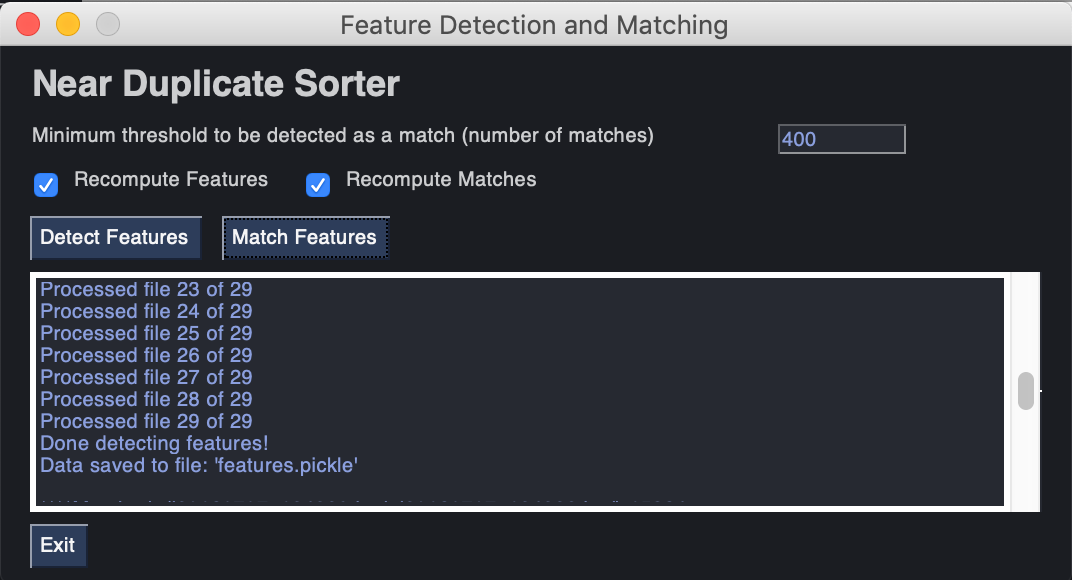
\includegraphics[width=1\textwidth]{images/near_duplicate_GUI1.png}
	\end{subfigure}%
	~
	\begin{subfigure}[b]{.5\textwidth}
		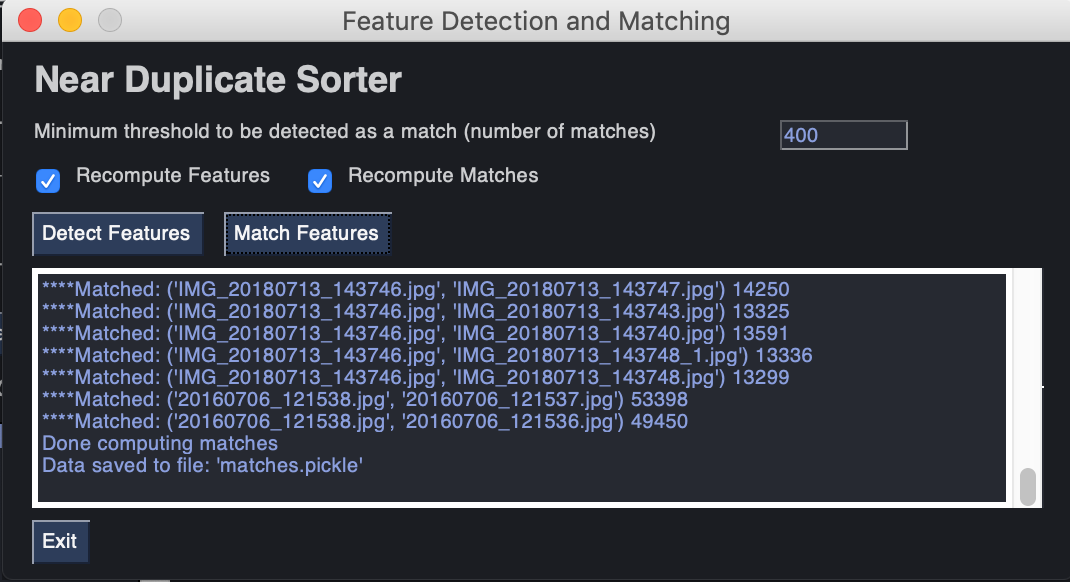
\includegraphics[width=1\textwidth]{images/near_duplicate_GUI2.png}
	\end{subfigure}

	\caption{Near Duplicate Sorter GUI running feature detection (left) and matching (right).}
		\label{fig:sort_gui}
\end{figure}

\begin{figure}[H]
	\centering
	\begin{subfigure}[b]{.33\textwidth}
		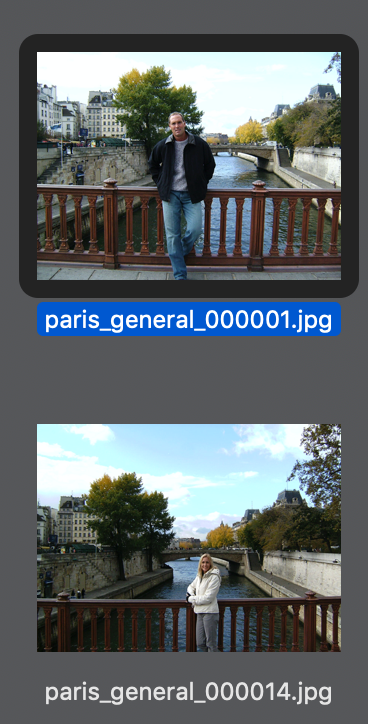
\includegraphics[width=.75\textwidth]{images/correct_match_1.png}
	\end{subfigure}%
	~
	\begin{subfigure}[b]{.33\textwidth}
		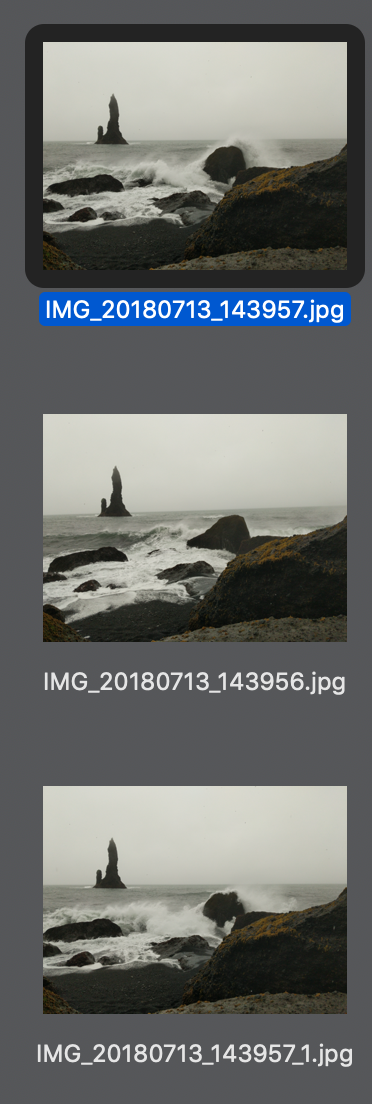
\includegraphics[width=.75\textwidth]{images/correct_match_3.png}
	\end{subfigure}%
	~
	\begin{subfigure}[b]{.33\textwidth}
		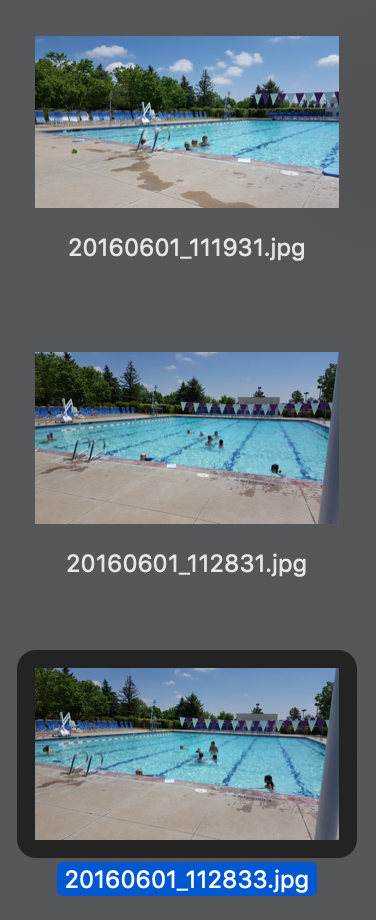
\includegraphics[width=.75\textwidth]{images/correct_match_4.png}
	\end{subfigure}

	\caption{Examples of properly sorted images}
	\label{fig:correct_sort}
\end{figure}

\begin{figure}[H]
	\centering
	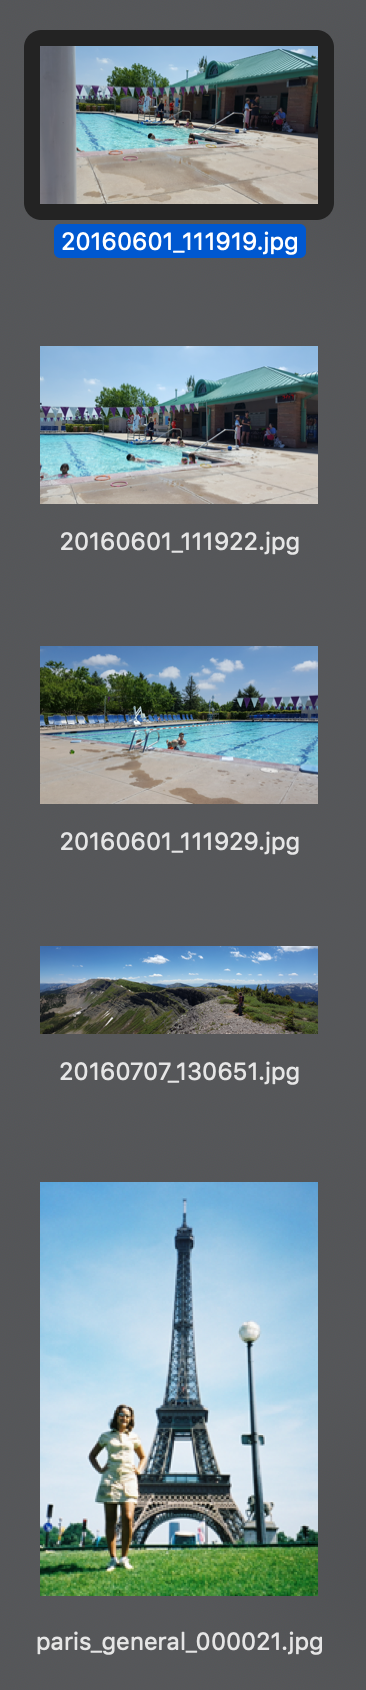
\includegraphics[width=.2\textwidth]{images/wrong_match_1.png}
	\caption{An example of a set of images that were improperly sorted.}
	\label{fig:incorrect_sort}
\end{figure}

	As you can see from Figure \ref{fig:incorrect_sort}, the algorithm is not perfect in any way. It can get very confused by images with similar background or similar regions of background. In the case of Figure \ref{fig:incorrect_sort}, the algorithm is most likely detecting the large sky components of the image that are bordered by trees/green grass as matching and so they get clustered together. By adjusting the sorting threshold higher than it was set (400 for these images), you could manually force the incorrect matches out into their own clusters. In doing this however, it is likely that other images don't match together than should as this threshold is not perfect and the higher it is the less likely images are to have enough feature matches to be clustered together.

\subsection{Image Sorter Timing}
	We also performed a very quick and basic runtime analysis of our program. The following data shows the runtime for our normal and matrix versions of the algorithm on 15 images and 50 images with various parameters.
	
	%. A longer analysis could be performed, however it would take a large amount of time to run permutations with more images and would show a very similar trend (just at larger scale).
	
	\begin{table}[H]
	\begin{adjustbox}{width=\columnwidth,center}
		\begin{tabular}{|c|c|c|c|c|}
			\hline
			\textbf{Algorithm Type} & 	\textbf{Number of Images} & 	\textbf{Recompute Features} & 	\textbf{Recompute Matches} & 	\textbf{Time (Seconds)} \\ \hline
			Normal & 15 & True & True & 63.152 \\ \hline
			Matrix & 15 & True & True & 127.498 \\ \hline
			Normal & 15 & False & True & 39.247 \\ \hline
			Matrix & 15 & False & True & 107.123 \\ \hline
			Normal & 15 & False & False & 0.663 \\ \hline
			Matrix & 15 & False & False & 0.562 \\ \hline
		\end{tabular}
	\end{adjustbox}
	\end{table}

\begin{table}[H]
	\begin{adjustbox}{width=\columnwidth,center}
		\begin{tabular}{|c|c|c|c|c|}
			\hline
			\textbf{Algorithm Type} & 	\textbf{Number of Images} & 	\textbf{Recompute Features} & 	\textbf{Recompute Matches} & 	\textbf{Time (Seconds)} \\ \hline
			Normal & 50 & True & True & 1613.024 \\ \hline
			Matrix & 50 & True & True &  ???? \\ \hline
			Normal & 50 & False & True & ???? \\ \hline
			Matrix & 50 & False & True &  ???? \\ \hline
			Normal & 50 & False & False & ???? \\ \hline
			Matrix & 50 & False & False &  ???? \\ \hline
		\end{tabular}
	\end{adjustbox}
\end{table}

	As the timing results show, the majority of the runtime is spent on the feature matching, as loading the features only reduces runtime by 37.85\% whereas loading both features and matches reduces it by 98.95\% for the normal version of the algorithm. For the matrix version of our algorithm, these were a 15.98\% and 99.56\% reduction respectively. This shows that the ability to save the number of matches between images is very beneficial to optimizing runtime. Our matrix implementation lets you take advantage of this reduction to half a second runtime when tuning the threshold, as it will always be around this runtime despite changing the threshold (with the assumption that you are not recalculating the matrix). With the normal implementation, if you changed the threshold it would take another 107 seconds to recompute the required matches every time, with no way to get around this forced re-computation.


\section{Analysis}

\subsection{Individual Contribution}
	

\subsection{Lessons Learned}
	The first lesson we learned with this project was that we should always use small data sets. We attempted to do a full test of the feature detection and matching after it was implemented and it took more than an hour to run. This was prompted by thinking the algorithm would run more efficiently than it did originally. After this first run, we cut the data set down for all out testing to 10-20 images and then increased it to 50-70 once we knew it was working and had implemented a few optimizations.
	
	Along a similar line, the second lesson we learned was that runtime matters a lot more than we thought it would. We had assumed that the functions would be a bit slow, but that running them on hundreds of images wouldn't be too bad and it really would only slow down once it hit many more than that. It turned out that even running it on just 15 images took between 1-2 minutes to run (depending on which version of the algorithm we used). This meant that when this was scaled up to hundreds of images it took incredible long times to run. The main solution to this was adding a couple optimizations to the code and the future plan of trying to multi-thread the application to allow it to do these computations faster. It was difficult to get around this one as a lot of the runtime was in library functions that we had no control over besides how many times we called them.
	
	A third lesson that we learned from this assignment is that it is very difficult to train a neural net well. You can train it on one thing, but it will likely be really bad at another. As such, we found that someone else has almost always trained a better neural net than we could for their own research or work. We learned that it is usually a good stepping stone to start with someone else's pre-trained network and the build from there to fit it to our own needs as they will have spent more time on the training and design than we would be able to for a single class.

\subsection{Advice for Future Students}
	Some advice that we would give next year's computer vision students is to explore different concepts with this project. There are many ways to do accomplish the same thing with computer vision and so they should not be afraid to try a bunch of different methods. Some of these methods wont work at all, some will work okay and others will be the best that research has produced. By trying a bunch of different thing that others have implemented before, you realize what they where made to specialize in and why people used them. In addition, it helps show you why people found better ways to do the same tasks better than if you just looked at them on the surface level.


\section*{References}
	As part of our object detection logic, we used pre-trained MobileNet-SSD model and prototext files to initialize our network. This specific MobileNet SSD was pre-trained on the Common Objects in Context dataset, and fine-tuned on the PASCAL Visual Object Classes dataset to get a mean average precision of around 72\%. \\
	\url{https://github.com/chuanqi305/MobileNet-SSD}
	
	The MobileNet research paper was referenced as well in researching the best option for our object detection network. \\ \url{https://arxiv.org/pdf/1704.04861.pdf}
	
	We ran into an issue when trying to save OpenCV keypoints from the feature detection algorithm to a file. To solve this, we used the function in the second answer from the following stack overflow post on how to pickle OpenCV keypoints. \\ \url{https://stackoverflow.com/questions/10045363/pickling-cv2-keypoint-causes-picklingerror/48832618}
	
	
	We also modified and used the example code from this tutorial to display the matches of the features while testing the implementation. This code is not specifically used in our GUI but was used in testing and is still in the code if we wanted to have the GUI display the feature matches at any point in the future. \\
	\url{https://docs.opencv.org/4.5.2/d1/de0/tutorial_py_feature_homography.html}
	
	In addition to these two specifically, the OpenCV documentation was referenced heavily to familiarize ourselves with functions and the different options and parameters that are available for use. \\
	\url{https://docs.opencv.org/4.5.2}
	
	The PySimpleGUI documentation was referenced heavily in building the frontend GUI portion of our application. \\ \url{https://pysimplegui.readthedocs.io/en/latest}

\end{document}

